% Chapter 6 – Detailed Service Designs
% =============================================================
\def\chapdir{./Chapter06}

% -------------------------------------------------------------
\chapter{Detailed Service Designs} \label{ch:service-designs}

This chapter presents the detailed internal design of each micro-service that makes up the OllamaNet back-end.  For every service we discuss its purpose, API surface, data model, main interaction flows, noteworthy implementation details, and how it integrates with the wider platform.

The phrase “AI model” was updated to “LLM” throughout, in line with the global terminology change.

% =============================================================
\section{AdminService}
\subsection{Purpose \& Responsibility}
AdminService is the administrative control centre of OllamaNet.  It offers
\begin{itemize}
  \item \textbf{User administration} – create, update, suspend and delete user accounts as well as manage role assignments;
  \item \textbf{LLM management} – register, edit and delete models plus meta-data and tags;
  \item \textbf{Tag management} – maintain the classification taxonomy;
  \item \textbf{Inference operations} – trigger model installation / removal on the InferenceService.
\end{itemize}

\subsection{API Design}
The REST endpoints are grouped by bounded context.  Selected examples are shown below.
\begin{itemize}
  % User Ops
  \item \textbf{GET} \texttt{/api/Admin/UserOperations/Users} – list users with pagination;
  \item \textbf{POST} \texttt{/api/Admin/UserOperations/Users} – create a new user;
  \item \textbf{PATCH} \texttt{/api/Admin/UserOperations/Users/\{id\}/Status} – change status.
  % LLM Ops
  \item \textbf{POST} \texttt{/api/Admin/AIModelOperations/Models} – register LLM;
  \item \textbf{DELETE} \texttt{/api/Admin/AIModelOperations/Models/\{id\}} – remove LLM.
  % Inference Ops
  \item \textbf{POST} \texttt{/api/Admin/InferenceOperations/Models/\{name\}/Pull} – pull model to inference node.
\end{itemize}
All endpoints enforce JWT authentication, FluentValidation rules and produce standardised problem-details responses.

\subsection{Data Model}
Key entities:
\begin{itemize}
  \item \textbf{ApplicationUser}, \textbf{Role}, \textbf{UserRole};
  \item \textbf{LLM}, \textbf{ModelVersion};
  \item \textbf{Tag}, \textbf{ModelTag} (many-to-many link).
\end{itemize}
The Repository pattern plus a Unit-of-Work orchestrates persistence.

\subsection{Sequence Diagrams}
The main flows are represented by Mermaid diagrams in the source markdown.  Place-holder images have been generated in \texttt{\chapdir/figures}.  For example:
\begin{figure}[h]
    \centering
    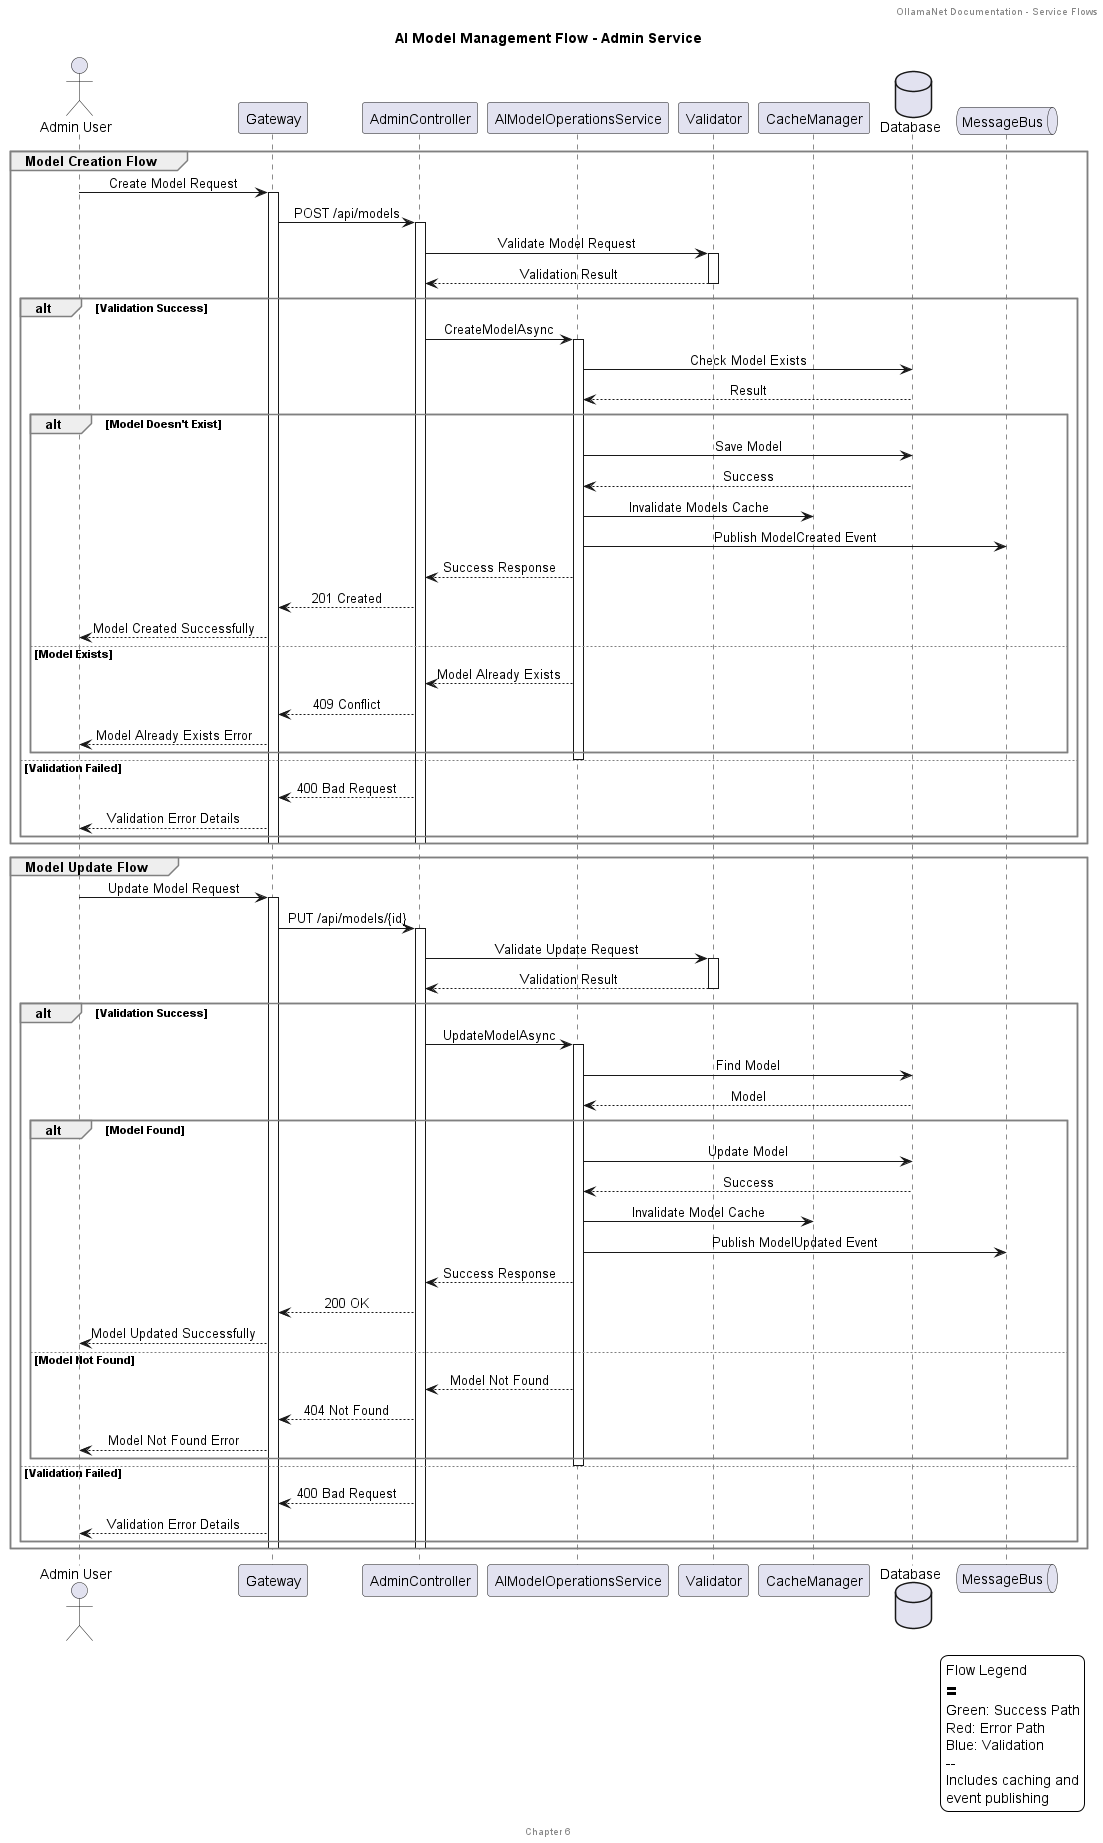
\includegraphics[width=\textwidth]{\chapdir/figures/adminservice_model_management_flow.png}
    \caption{AdminService – LLM management flow}
    \label{fig:adminservice-model-flow}
\end{figure}

\subsection{Service-specific Components}
\begin{itemize}
  \item \emph{CacheManager} + Redis two-tier cache.
  \item Ollama integration client for on-demand model installation.
  \item Message handlers for RabbitMQ service-discovery events.
\end{itemize}

\subsection{Integration Points}
AdminService interacts with:
\begin{itemize}
  \item AuthService (JWT validation);
  \item InferenceService (model install / delete APIs);
  \item RabbitMQ (broadcast inference URL changes).
\end{itemize}

% =============================================================
\section{AuthService}
\subsection{Purpose \& Responsibility}
AuthService secures the platform by handling authentication and authorisation.  It issues short-lived JWTs and manages refresh tokens via secure HTTP-only cookies.

\subsection{API Design}
\begin{itemize}
  \item \textbf{POST} \texttt{/api/Auth/Login} – user login (JWT + refresh cookie);
  \item \textbf{POST} \texttt{/api/Auth/Refresh} – obtain new JWT;
  \item \textbf{POST} \texttt{/api/Auth/Register} – create account.
\end{itemize}

\subsection{Data Model}
\begin{itemize}
  \item Identity entities: \textbf{ApplicationUser}, \textbf{Role}, \textbf{RefreshToken}.
\end{itemize}

\subsection{Sequence Diagrams}
\begin{figure}[h]
    \centering
    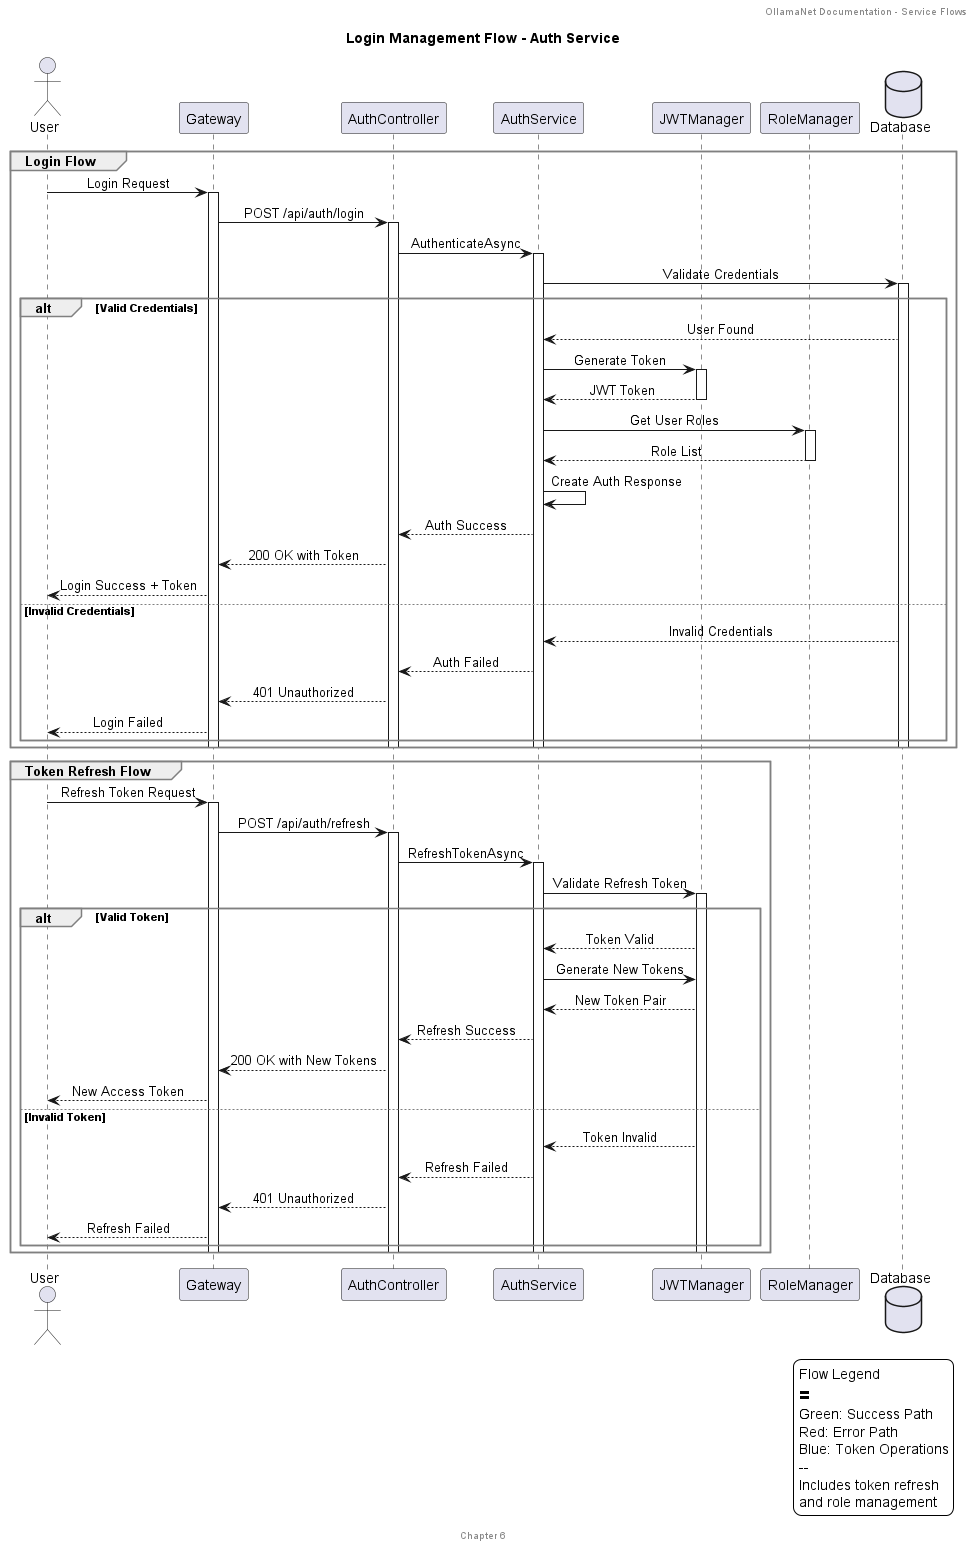
\includegraphics[width=\textwidth]{\chapdir/figures/authservice_login_flow.png}
    \caption{AuthService – Login flow}
\end{figure}

\subsection{Service-specific Components}
\begin{itemize}
  \item Password hashing with ASP.NET Core Identity;
  \item Refresh-token rotation with revocation list;
  \item Email sender for verification / reset.
\end{itemize}

\subsection{Integration Points}
Consumes AdminService role data; issues JWTs to every other service.

% =============================================================
\section{ExploreService}
\subsection{Purpose \& Responsibility}
Allows users to discover, filter and search available LLMs.

\subsection{API Design}
\begin{itemize}
  \item \textbf{GET} \texttt{/api/Explore/Models} – list models (pagination, filter by tag);
  \item \textbf{GET} \texttt{/api/Explore/Models/\{id\}} – detailed model info.
\end{itemize}

\subsection{Data Model}
\begin{itemize}
  \item \textbf{LLM}, \textbf{Tag}, \textbf{ModelTag} relationships.
\end{itemize}

\subsection{Sequence Diagrams}
\begin{figure}[h]
    \centering
    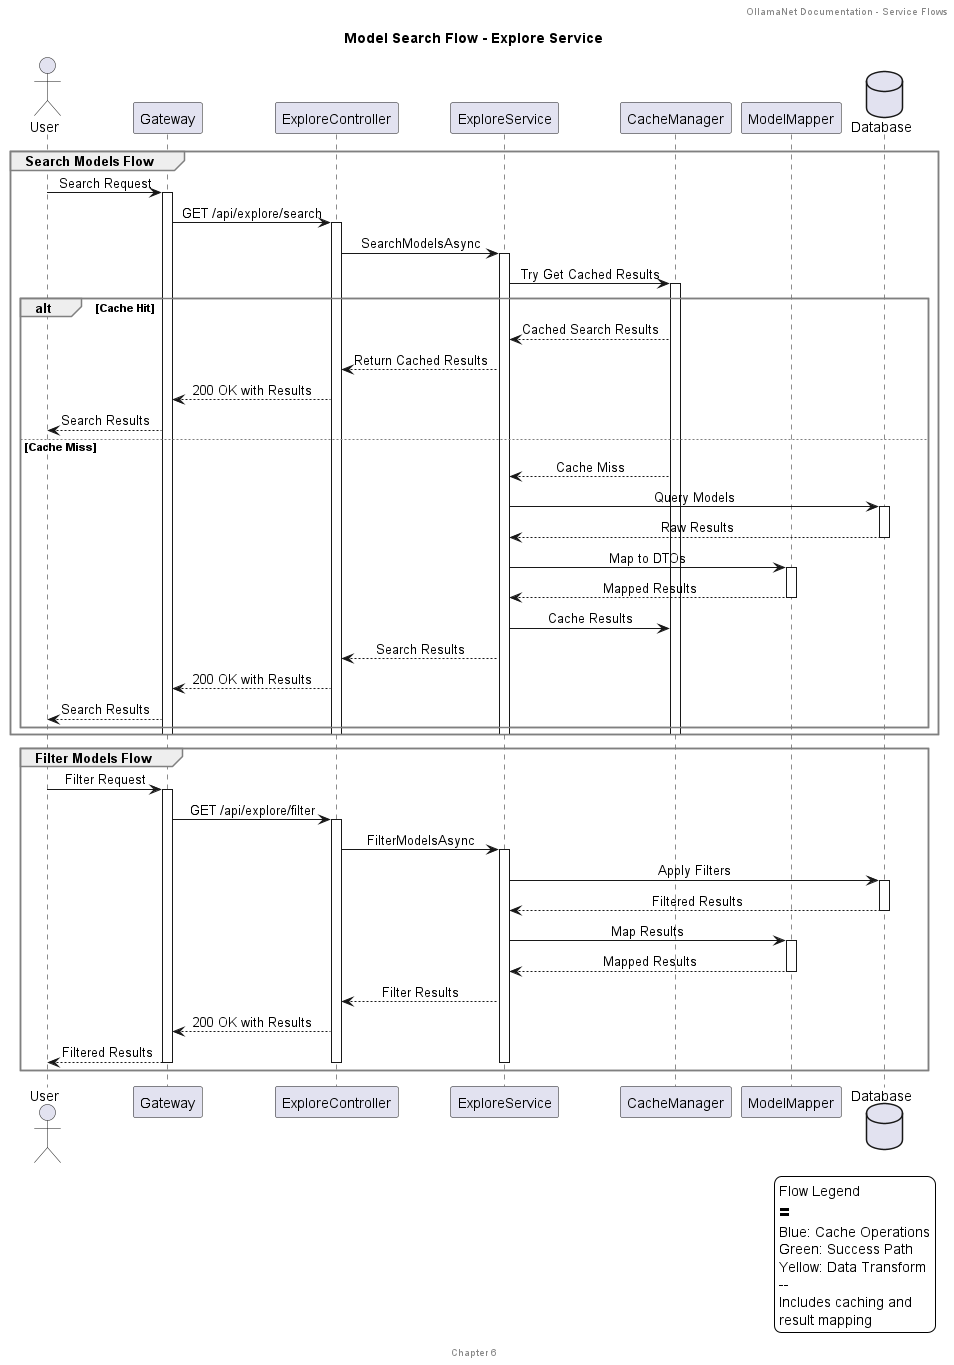
\includegraphics[width=\textwidth]{\chapdir/figures/exploreservice_search_flow.png}
    \caption{ExploreService – Tag search flow}
\end{figure}

\subsection{Service-specific Components}
\begin{itemize}
  \item Redis-backed read-through caching;
  \item Domain exceptions hierarchy for robust error reporting.
\end{itemize}

\subsection{Integration Points}
Reads model catalog maintained by AdminService; exposed to UI / external clients.

% =============================================================
\section{ConversationService}
\subsection{Purpose \& Responsibility}
Manages chat threads, message storage, and conversation context for LLM sessions.

\subsection{API Design}
\begin{itemize}
  \item \textbf{GET} \texttt{/api/Conversation/Conversations} – list conversations;
  \item \textbf{POST} \texttt{/api/Conversation/Conversations} – create conversation.
\end{itemize}

\subsection{Data Model}
Entities: \textbf{Conversation}, \textbf{Message}, \textbf{Attachment}, \textbf{LLMResponse}.

\subsection{Sequence Diagrams}
% Placeholder figure commented out.

\subsection{Service-specific Components}
\begin{itemize}
  \item Repository layer with soft-delete for messages;
  \item Saga-style workflow coordinating message save and inference call.
\end{itemize}

\subsection{Integration Points}
Calls InferenceService for streaming completions; publishes events to NotificationService (future work).

% =============================================================
\section{InferenceService}
\subsection{Purpose \& Responsibility}
Hosts the local Ollama engine and exposes HTTP endpoints (proxied by ngrok) for text generation.

\subsection{API Design}
\begin{itemize}
  \item \textbf{POST} \texttt{/api/chat} – single request/response completion;
  \item \textbf{POST} \texttt{/api/chat?stream=true} – streaming completion.
\end{itemize}

\subsection{Service-specific Components}
\begin{itemize}
  \item Notebook-based process manager that boots Ollama and ngrok;
  \item RabbitMQ publisher announcing public URL updates.
\end{itemize}

\subsection{Integration Points}
Consumed by ConversationService and AdminService.

% =============================================================
\section*{Glossary}
\begin{description}
  \item[AdminService] Platform administration micro-service.
  \item[AuthService] Authentication / authorisation micro-service.
  \item[ExploreService] Model discovery micro-service.
  \item[ConversationService] Chat and message management micro-service.
  \item[InferenceService] Ollama-powered text generation micro-service.
  \item[LLM] Large Language Model.
  \item[RabbitMQ] Message broker used for service-discovery events.
\end{description}
